\newpage
\subsection{Connecting your classes}
\genHeader
\hypertarget{static:references splash}{}

\texttt{}
\emph{}

At this point, you've declared your types and attributes, but what good are those if nothing can communicate with something else? We need to create some
\emph{EReferences}!

There are 3 properties that must be set in order to create an EReference: \emph{Navigation}, \emph{Aggregation}, and
\emph{Multiplicity}. As you can probably guess, they're declared differently in each syntax, but let's review the concepts since they're the same.

Firstly, \texttt{Navigable} ends are mapped to class attributes with getters and setters in Java, and therefore \emph{must} have a specified name and
multiplicity for successful code generation. Corresponding values for \texttt{Non-Navigable} ends can  be regarded as additional documentation, and do not have
to be specified.

Second, the \texttt{Multiplicity} refers to that of a reference\footnote{Don't get multiplicity of a reference confused with the multiplicity of an element!
Multiplicity of an element defines the permitted range of individual instances, rather than classes.}. It controls if the relation is mapped to a
Java Collection (\texttt{*},~\texttt{1..*},~\texttt{0..*}), or to a single valued class attribute (\texttt{1}, \texttt{0..1}). We'll explain this setting in
detail when you encounter them in your syntax instructions.

Lastly, in Ecore, the \texttt{Aggregration} values of a reference can be \texttt{none}, \texttt{shared}, or \texttt{com\-po\-site}. Composite means that the
current role is that of a \emph{container} for the opposite role. You'll see in our example that \texttt{Box} is a container for several \texttt{Partition}s.
This has a series of consequences: (1) every element must have a container, (2) an element cannot be in more than one container at the same time, and (3) a
container's contents are deleted together with the container. Conversely, non-composite (\texttt{none}) means that the current role is not that of a container,
and the rules for containment do not hold (in other words, the reference is set a simple `pointer'). The \texttt{shared} setting is beyond the scope of this
handbook.


\fancyfoot[RO]{ $\triangleright$ \hyperlink{static:references vis}{Next [visual]\hspace{0.2cm}} \\ $\triangleright$ \hyperlink{static:references tex}{Next
[textual]}}

\newpage
\subsubsection{Creating EReferences in EA}
\visHeader
\hypertarget{static:references vis}{}

\begin{itemize}

\item[$\blacktriangleright$] A fundamental gesture in EA is \emph{Quick Link}. Quick Link is used to create EReferences between elements in a context-sensitive
manner. To use quick link, choose an element and note the little black arrow in its top-right corner (Fig.~\ref{fig:quicklink}).

\begin{figure}[htbp]
	\centering
  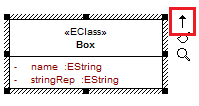
\includegraphics[width=0.4\textwidth]{ea_quickLink}
	\caption{Quick Link is a central gesture in EA}
	\label{fig:quicklink}
\end{figure}
\FloatBarrier

\item[$\blacktriangleright$] Click this black arrow and `pull' to the element you wish to link to. To start, quick-link from \texttt{Box} to \texttt{Partition}.
In the context menu that appears, select ``Create Bidirectional EReference'' (Fig.~\ref{fig:ereference}).

\begin{figure}[htbp]
	\centering
  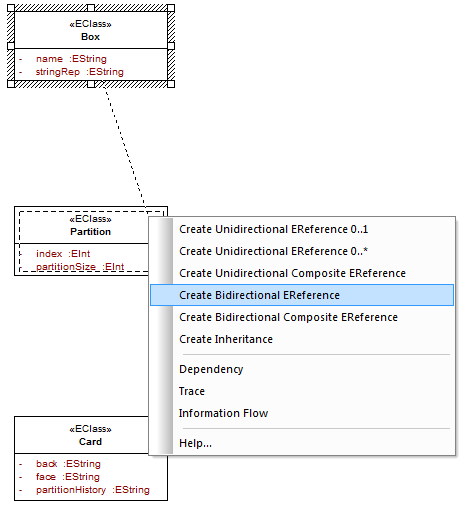
\includegraphics[width=0.6\textwidth]{ea_eReferenceBidirectional}
	\caption{Create an EReference via Quick Link}
	\label{fig:ereference}
\end{figure}
\FloatBarrier

\item[$\blacktriangleright$] Double click the EReference to invoke a dialogue. In this window you can adjust all relevant settings. Feel free to leave the
\texttt{Name} value blank - this property is only used for documentation purposes, and is not relevant for code generation.

\item[$\blacktriangleright$] Within this dialogue, go to ``Source Role,'' and compare the relevant values in Fig.~\ref{fig:role_source} for the \emph{source}
end of the EReference (the \texttt{Box} role). As you can see, the default source is set to the EClass you linked from, while the default target
is the EClass you linked to. In this window, do not forget to confirm and modify the \texttt{Role}, \texttt{Navigability}, \texttt{Multiplicity}, and
\texttt{Aggregation} settings for the source as required. Repeat the process for the \texttt{Target Role} (Fig.~\ref{fig:role_target}).

\vspace{0.5cm}

\begin{figure}[htbp]
	\centering
    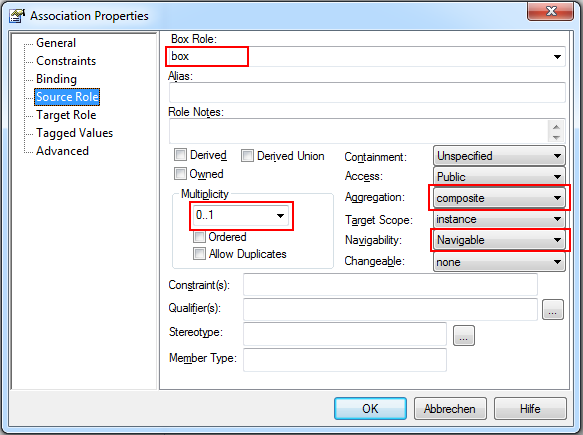
\includegraphics[width=0.9\textwidth]{ea_assocPropsSource}
	\caption{Properties for the source role of an EReference}
	\label{fig:role_source}
\end{figure}

\begin{figure}[htbp]
	\centering
	  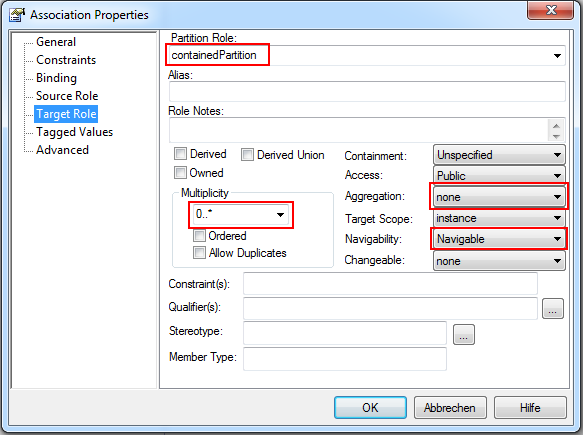
\includegraphics[width=0.9\textwidth]{ea_assocPropsTarget}
	\caption{Properties for the target role of an EReference}
	\label{fig:role_target}
\end{figure}

\end{itemize}

To review these properties, the first value you edited was the role name. The \texttt{Navigation} value should have been automatically set to
\texttt{Na\-vi\-ga\-ble}. Without these two settings, getter and setter methods will not be generated.

Next, you set the \texttt{Multiplicity} value.  In your source role (\texttt{Box}), you have allowed the creation of up to one target (\texttt{Partition})
reference for every connected source (\texttt{box}). This means you could not have a single target connected to two sources (i.e., one partition that belongs to
two boxes). In the target (\texttt{Partition}) role, you have specified that any source (in our case, \texttt{box}) can have any positive-sized number of targets.
Figure~\ref{fig:sketch_roles} sketches this schematically.

\vspace{0.5cm}

\begin{figure}[htbp]
	\centering
    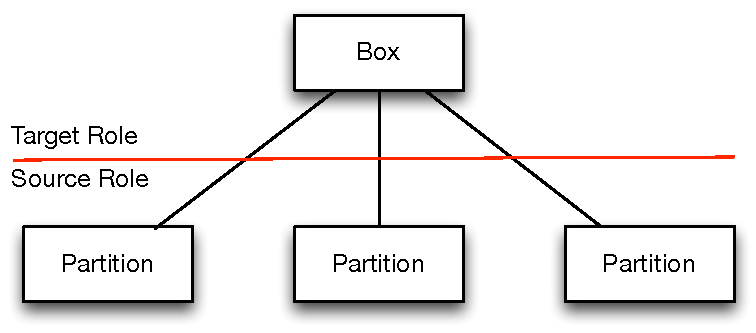
\includegraphics[width=0.6\textwidth]{sketch_multiplicities.pdf}
	\caption{The target and source roles of Leitner's Learning Box}
	\label{fig:sketch_roles}
\end{figure}
\FloatBarrier

Finally, you set the \texttt{Aggregation} value. In this case, \texttt{box} is a container for \texttt{Partition}s, and \texttt{containedPartition} is
consequently not.

\begin{itemize}
\item[$\blacktriangleright$] Take a moment to review how the \texttt{Aggregration} settings extend the \texttt{Multiplicity} rules. If you've done everything
right, your metamodel should now resemble Fig.~\ref{fig:ereference_completed}, with a single \emph{bidirectional EReference} between \texttt{Box} and
\texttt{Partition}.

\vspace{1cm}

\begin{figure}[htbp]
	\centering
  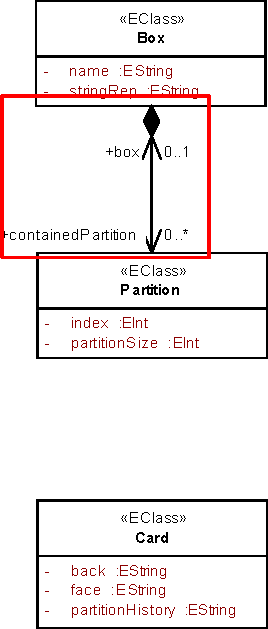
\includegraphics[width=0.35\textwidth]{ea_relationBoxPartition.pdf}
	\caption{\texttt{Box} contains \texttt{Partition}s}
	\label{fig:ereference_completed}
\end{figure}
\FloatBarrier

\item[$\blacktriangleright$] Following the same process, create two unidirectional self-EReferences for \texttt{Partition}, and then a second bidirectional
EReference\footnote{To be precise, \emph{all} EReferences in Ecore are actually unidirectional. A ``bidirectional'' EReference in our metamodel is really two
mapped EReferences that are opposites of each other. We however, believe it is simpler to handle these pairs as single EReferences, and prefer this
concise concrete syntax.} between \texttt{Partition} and \texttt{Card} (Fig.~\ref{fig:ereferences_all}). 

\vspace{1cm}

\begin{figure}[htbp]
	\centering
  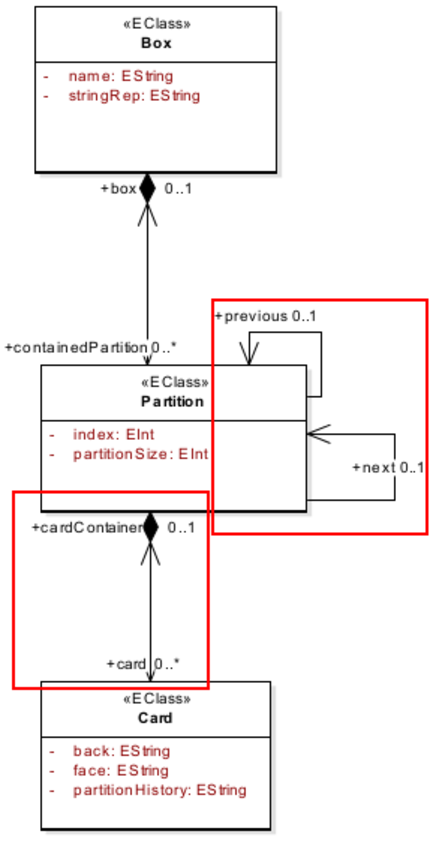
\includegraphics[width=0.7\textwidth]{ea_classAttributes}
	\caption{All relations in our metamodel}
	\label{fig:ereferences_all}
\end{figure}
\FloatBarrier

\vspace{1cm}

\item[$\blacktriangleright$] You'll notice that the connection between \texttt{Card} and \texttt{Partition} is similar to that between \texttt{Partition} and
\texttt{Box}. This makes sense as a partition should be able to hold an unlimited amount of cards, but a card can only belong to one partition at a time.

\vspace{1cm}

\item[$\blacktriangleright$] Export your diagram to Eclipse and refresh your workspace. Your Ecore file should now resemble Fig~\ref{fig:model_allClasses}.

\vspace{1cm}

\begin{figure}[htbp]
	\centering
  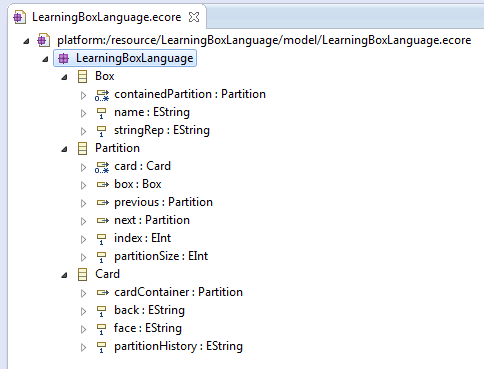
\includegraphics[width=0.7\textwidth]{eclipse_modelDeclaredClasses}
	\caption{Refreshed Ecore file with all EReferences}
	\label{fig:model_allClasses}
\end{figure}

\vspace{1cm}

\item[$\blacktriangleright$] All the required attributes and references for your learning box have now been set up. We encourage you to see how these are
declared in the textual syntax, starting on the immediate next page. In particular, check out Fig.~\ref{fig:allReferences}, where each EClass is fully
declared, and Fig.~\ref{fig:bothConstraints}, where bidirectionality is explicitly specified as a constraint.

\jumpSingle{static:methods vis}

\end{itemize}

\newpage
\subsubsection{Connecting your classes with MOSL}
\texHeader
\hypertarget{static:references tex}{}

In MOSL, the declaration of a reference is simple; the syntax is made up of four parts:  \small{\texttt{[Aggregation Type][Navigation
Name](Multiplicity):[Role]}}. A simple reference is defined with an arrow operator, while a contained reference is a sideways diamond and arrow combination.

% Edit me
To avoid redundancies in your code, it's important to know that both types automatically update the other role involved in the reference, which means you only
have to declare a direction once.


\begin{itemize}

\item[$\blacktriangleright$] Open \texttt{Box} class in the editor and add a \emph{container reference} named \texttt{containedPartition} with a multiplicity of zero
to infinite, of type \texttt{Partition} (Fig.~\ref{fig:cpartitionReference}). This means {\bf THAT}.

\begin{figure}[htbp]
	\centering
  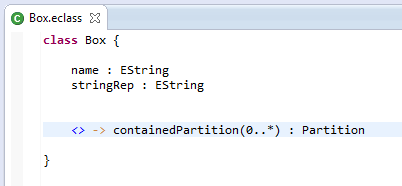
\includegraphics[width=0.6\textwidth]{eclass_box}
	\caption{Creating a \emph{contained reference} in \texttt{Box}}
	\label{fig:cpartitionReference}
\end{figure} 

\item[$\blacktriangleright$] Now add a \emph{simple reference} to \texttt{Partition}. Name it \texttt{box}, and allow it to hold up to one \texttt{Box}
(Fig.~\ref{fig:boxReference}). This means {\bf THAT}.

\begin{figure}[htbp]
	\centering
  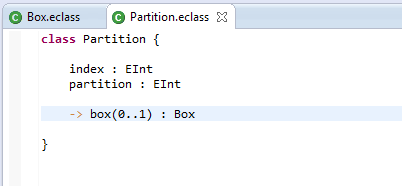
\includegraphics[width=0.6\textwidth]{eclass_partition}
	\caption{Creating a \emph{simple reference} in \texttt{Partition}}
	\label{fig:boxReference}
\end{figure} 

\item[$\blacktriangleright$] Congratulations, you have just built your first pair of EReferences. This pair is also known as a \emph{Bidirectional
EReference}! To see how this is depicted visually, check out Fig.~\ref{fig:ereference_completed} in the previous subsection.

\newpage

\item[$\blacktriangleright$] Now, lets create another EReference pair, or bidirectional EReference, between \texttt{Partition} and \texttt{Card}. If you think
about it, it's really not all that different than the relation between \texttt{Box} and \texttt{Partition}. In fact, it's not different at all! A
\texttt{Partition} should be able to hold an unlimited amount of \texttt{Card}s, but a \texttt{Card} should only be allowed to belong to zero or one
\texttt{Partition}s. Name the two new relations \texttt{containedPartition}, and \texttt{box}.

\item[$\blacktriangleright$] Your classes should now closely resemble Fig.~\ref{fig:almostAllReferences}.

\begin{figure}[htbp]
	\centering
  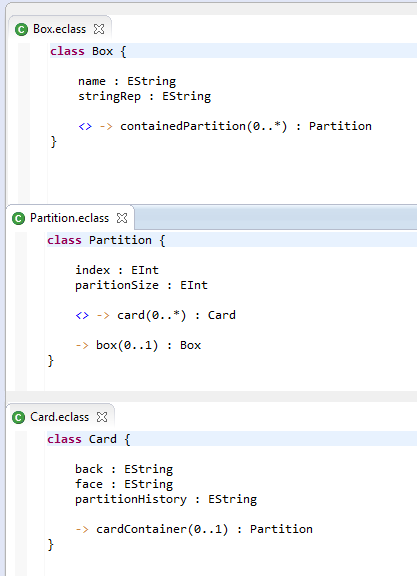
\includegraphics[width=0.65\textwidth]{eclipse_workspaceReferences}
	\caption{The Completed Bidirectional EReferences}
	\label{fig:almostAllReferences}
\end{figure} 

\item[$\blacktriangleright$] The next step is to set up two relations between \texttt{Partition} and itself, so it can shift between the previous and next
partition in the box. Create two new simple references, named \texttt{previous}, and \texttt{next}. Allow them to have a maximum of 1 link each.

\item[$\blacktriangleright$] All of our references are now set up! If you have done everything correctly, your classes should now resemble Fig.~\ref{fig:allReferences}.
To see how all of this is depicted visually, check out Fig.~\ref{fig:ereferences_all} in \hyperlink{sec:static vis}{section 2.1}.

\begin{figure}[htbp]
	\centering
  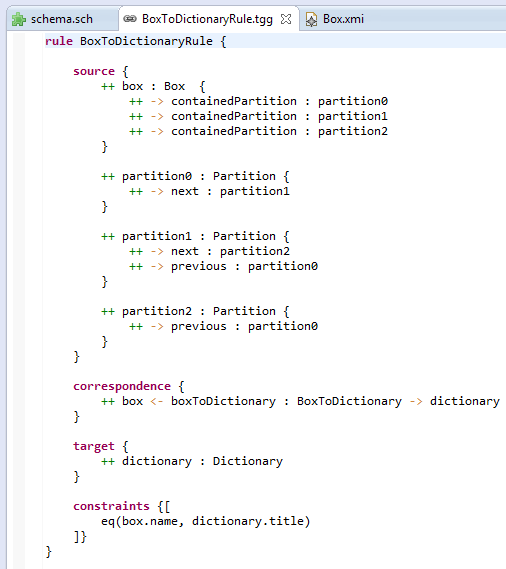
\includegraphics[width=0.6\textwidth]{eclipse_allReferences}
	\caption{All references in Leitner's Learning Box}
	\label{fig:allReferences}
\end{figure} 

\fancyfoot[R]{$\triangleright$ \hyperlink{static:methods tex}{Next}}
\end{itemize}

